%!TEX root = ../thesis_phd.tex
%%%%%%%%%%%%%%%%%%%%%%%%%%%%%%%%%%%%%%%%%%%%%%%%%%%%%%%%%%%%%%%%%%%%%%%%%%%%%%%%
% simulation.tex: Chapter on MC production:
%%%%%%%%%%%%%%%%%%%%%%%%%%%%%%%%%%%%%%%%%%%%%%%%%%%%%%%%%%%%%%%%%%%%%%%%%%%%%%%%
\chapter{Monte Carlo Simulation}
\label{sim_chapter}
%%%%%%%%%%%%%%%%%%%%%%%%%%%%%%%%%%%%%%%%%%%%%%%%%%%%%%%%%%%%%%%%%%%%%%%%%%%%%%%%


The \nova Monte Carlo (MC) simulation chain involves many components to deliver an accurate representation; starting with protons on the \numi target and running all the way through APD readout in the \nova detectors.  FLUKA and FLUGG are used to simulate the flux in the NuMI beamline \cite{fluka}.
Neutrino interactions within the detectors are simulated using \genie
\cite{genie}.
\geant is used to propagate products of the neutrino interactions through a detailed model of the \nova~detectors \cite{geant}
Custom NOvA simulation software converts energy depositions into electronic signals \cite{aurisano2015nova}.
While this chapter aims to describe the methods involved in simulating detector effects, it also provides a detailed description of the
effects themselves.


\section{Beam Simulation}
\label{beam_sim_section}

The \numi beam simulation is used to predict the neutrino flux
in both the ND and FD.
Simulated protons from the Main Injector are directed upon a model of the
target and its surroundings; the resulting shower of hadrons
is tracked in detail in order to predict neutrino production.

While the absolute flux is predicted in both detectors,
it is really the ratio of the predicted fluxes which enters into an oscillation
analysis.
ND data are extrapolated to the FD to mitigate systematic errors
the absolute flux estimate, so the beam simulation mainly serves
to transfer the observed ND spectrum into an FD prediction.
The extrapolation procedure will be described in detail in Section
\ref{extrap_section}, although it should be noted here that the primary
difference in the fluxes seen between the two detectors arise from geometric
effects.
The ND is close to the \numi source; despite its relatively small size,
it subtends a much larger solid angle, and thus a spectrum of incident
neutrino angle and energy.
Also note that the detectors themselves do not observe the neutrino flux
directly, but rather its convolution with cross section, which is discussed
in the following section.

A detailed representation of the \numi target facility forms the basis
of beam simulation.
The geometry of the target hall is encoded in the \geant geometry format
to capture the positions and compositions of the target, collimator,
focusing horns, and decay pipe.
The FLUKA \cite{fluka} particle simulation package is used to track the
ancestry of hadrons through the target and their decay downstream.
An interface between FLUKA and the \geant geometry is provided
by  FLUGG \cite{campanella1999first}.
In this framework, neutrinos produced in the beam can be traced back
through the hadronization chain to the primary proton which interacted in the
target.
Such precision allows detailed studies to estimate uncertainties based
on particle production and interaction models.
The FLUKA/FLUGG simulation has been cross-checked by an independent
\geant simulation (based on the same geometry) and shown to produce
comparable results.
Comparisons have also been made to data both from the NA49
\cite{gazdzicki2004report} and MIPP \cite{paley2014measurement}
experiments in order to estimate systematic errors.

The output of the beam simulation is a representation of the \numi flux
in terms of flavor and momentum which can be passed to downstream simulation
components.  A depiction of the observed event rate in both detectors can be
seen in Figure \ref{beam_flux_fig}.

\begin{figure}
\begin{center}
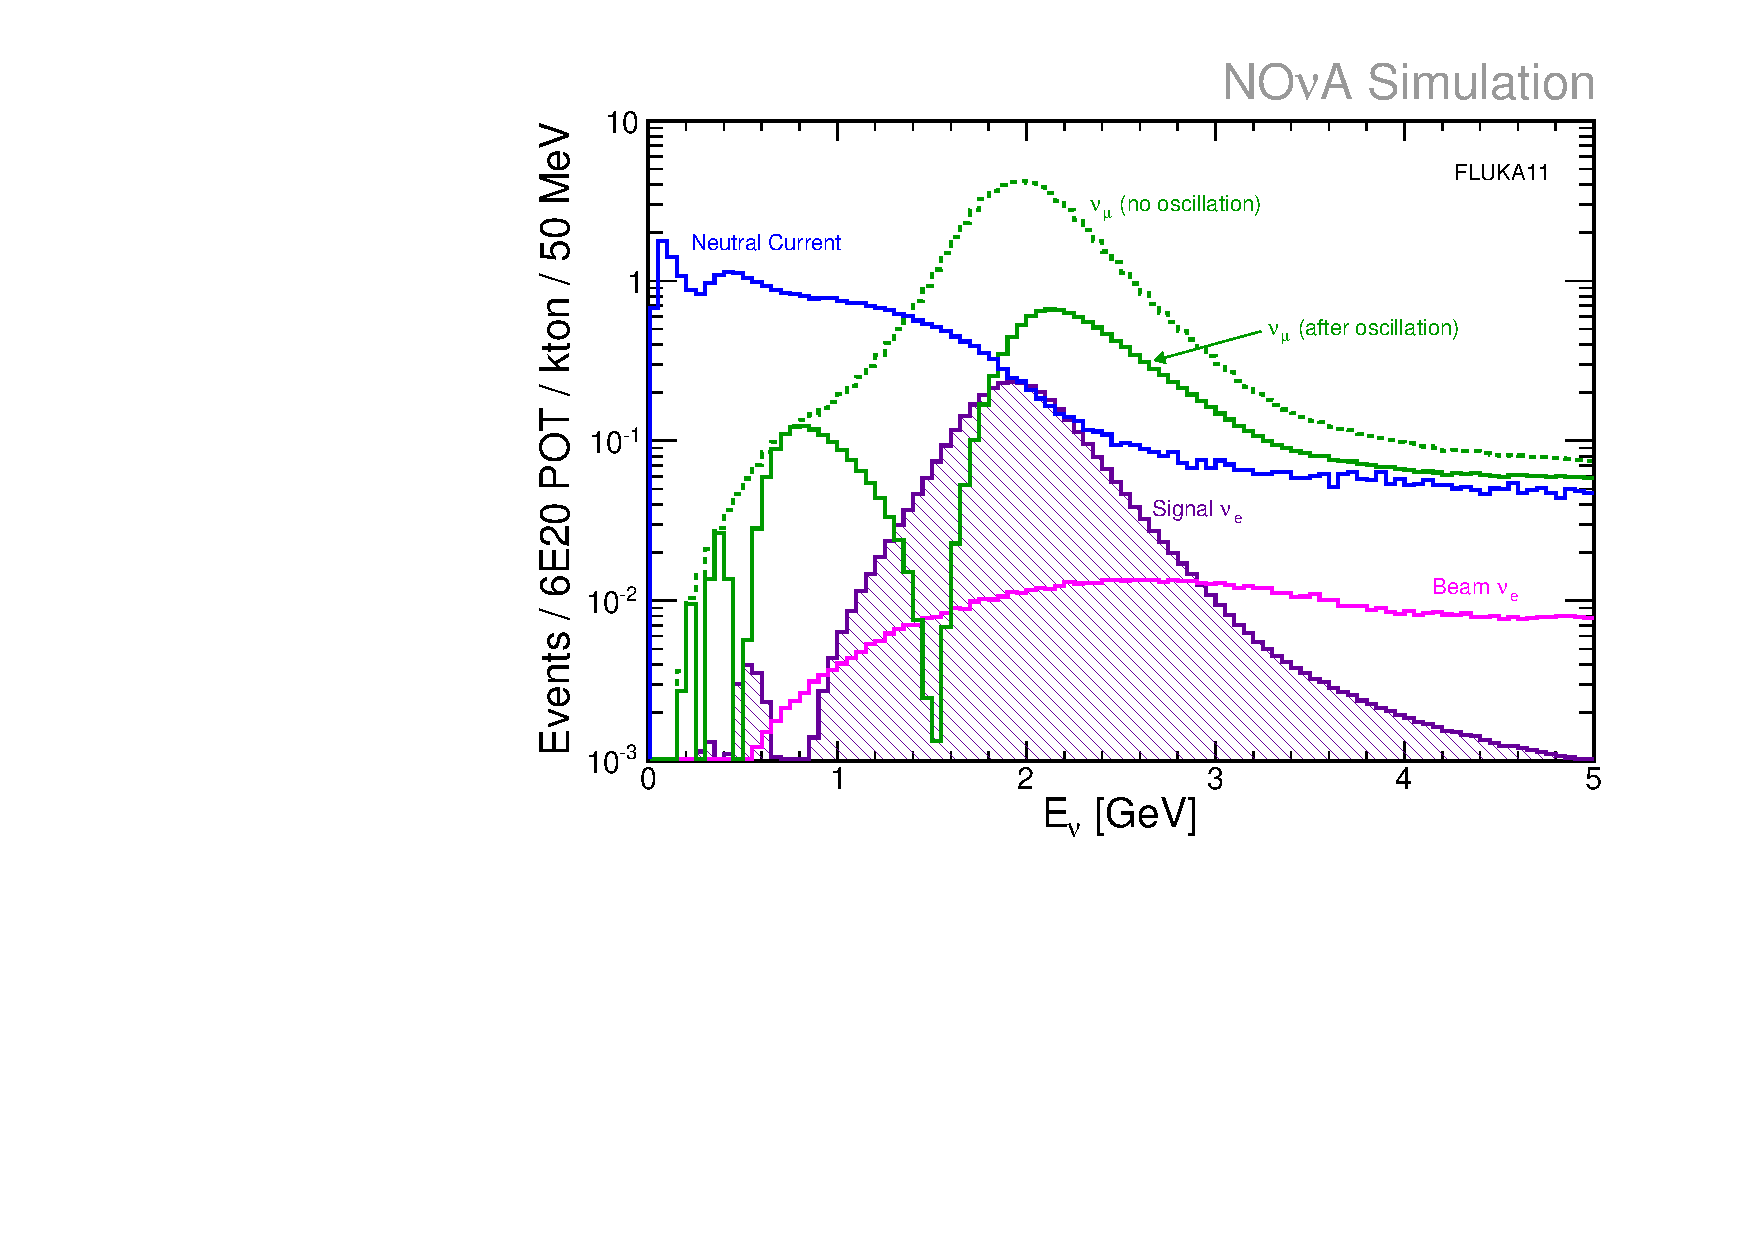
\includegraphics[width=\textwidth]{figures/plots/nova/beam_flux_log.pdf}
\end{center}
\caption{Simulated spectrum of observed FD events}{
The observed neutrino event spectrum in \nova is the convolution
of \numi beam flux and neutrino interaction cross section.
The spectra here show the predicted rate of neutrino interactions
in \nova as a function of interaction energy.
Depicted in green is the \numu CC interaction spectrum; the dashed line
is the prediction in the absence of neutrino oscillation, while
the solid line includes the effect.
The purple distribution shows the appeared \nue CC spectrum,
while the magenta distribution shows the intrinsic \nue component
of the beam.
NC events, shown in blue, are binned in terms of their visible energy
(excluding the energy of the outgoing neutrino) in order to represent
the energy which would be deposited in the detector.
}
\label{beam_flux_fig}
\end{figure}



\section{\genie -- Neutrino Interaction Simulation}
\label{genie_section}

\genie is a comprehensive neutrino MC generator for the experimental physics community.
According to the \genie collaboration mission statement, the
generator aims to simulate processes  for all neutrino species and all nuclear targets, from the MeV to PeV scale.  The input to GENIE is the simulated detector flux from FLUKA/FLUGG; the output is a collection of neutrino interactions described as \genie event records.  \genie event records catalog the flavor and kinematics of the incoming neutrino, struck nucleus, and daughter particles which leave the nucleus.

Nuclear structure is at the core of neutrino interaction simulation, for which
\genie uses the Relativistic Fermi Gas model of Bodek and Ritchie
\cite{bodekritchie}.
At low energies, this gives a reasonable approximation of nuclear binding
energies and struck nucleon momentum.
At higher energies, it provides a model for nuclear shadowing and other
effects.


A principal component in neutrino event generation is interaction cross sections.  In order to generate events across such a wide range of energies, \genie must stitch together a variety of cross section models.  \genie calculates a total cross section by integrating over the differential cross sections from the various models.  The total cross section is combined with the flux (from FLUKA and FLUGG simulations in this case) and detector geometry to produce the overall energy spectrum of interacting neutrinos.
Since this step is relatively computationally expensive, \genie computes the
energy spectra as a separate process and stores the interpolated result
based upon cubic splines \cite{atkinson1978introduction}.
For each generated event, the energy splines are sampled to select the interaction energy, but differential cross sections are used to sample the remaining kinematics.

While \genie employs several cross section models, only a
few are important for this work.
The selected \numu CC events in \nova are dominated by just three interaction modes: Quasi-Elastic scattering (QE),  baryon resonance production (RES) and deep-inelastic scattering (DIS).
QE interactions can be interpreted as a neutrino scattering off a single
nucleon, RES interactions involve an excitation
of the nucleus by the neutrino, and DIS represented as an interaction
with the entire nucleus which can induce complete
nuclear disintegration.
QE events dominate the low energy tail of the energy spectrum, while DIS events account for most of the high energy tail.

The QE model in \genie is an implementation of the Llewellyn-Smith model \cite{LlewellynSmith} with a dipole form factor.  In that implementation, the axial vector mass is the sole free parameter.  RES events are generated using from the Rein-Segal model \cite{rein1981neutrino}, which employs the Feynman-Kislinger-Ravndal (FKR) model of baryon resonances \cite{feynman1971current}.  FKR parameterizes resonance
wave functions as excited states of a 3-quark system in a relativistic harmonic
oscillator potential.  The \genie implementation of Rein-Segal neglects interference between resonances as well as outgoing lepton masses.  Similar to the QE model, this RES implementation leaves the axial vector mass.  For DIS interactions, \genie uses a leading order model with corrections from Bodek and Yang \cite{bodek2003higher} to better describe the low $Q^2$ region.  This crossover energy region where DIS interactions begin to dominate is of principal importance to \nova since it accounts for most of the events on the high side of the energy peak.  \genie calculates DIS cross sections at the parton level, or in other words, the cross section involves all sea and valence quarks.  This implementation of DIS involves many free parameters, although most of them have small effects on the \numu CC event selection in \nova.

Free parameters in \genie will be discussed further in chapter \ref{systs_chapter}.  For now, it is important to note that \genie includes a reweighting feature or all free parameters in the models it includes.  For any given event, a weight can be determined by calculating the cross section with a modification of one of the free parameters.  The weights are calculated simply by taking the ratio of this modified cross section to the original cross section.


\section{\geant -- Interaction Product Propagation}
\label{geant_section}
\geant \cite{geant} is a popular software suite for simulating the passage of
particles through matter.  In the \nova simulation chain, \genie produces
daughter particles leaving the nucleus, then \geant simulates the passage of
those particles through matter.  \geant is thus responsible for the energy
deposition, interaction and decay of those particles within the detector and
surrounding materials.

This propagation relies on a detailed representation of the detector geometry which the describes the position of assorted materials.
The locations of the blocks have been taken from the as-built locations measured by a laser scan system, although it does not include the precisely measured tilt and stager on a plane-by-plane basis.
Certain features are impossible or difficult to measure and incorporate into
the geometry, for instance the location of the fiber within the cells and glue voids between modules.  The geometry also includes materials surrounding the detector.  These materials include the steel support structure around the detectors, the rock and concrete comprising the detector halls, as well as the overburden above the FD.

The models which govern interaction, energy deposition and decay of particles in GEANT is highly configurable through so-called \textit{physics lists}.  \nova simulation uses the QGSP\_BERT\_HP physics list by default; although other physics lists have been used to study systematic effects, namely FTF\_BIC, QGSP\_BIC\_HP and QGSC\_BERT.  QGS refers to the quark-gluon string model for hadronic interactions above 20 GeV \cite{kaidalov1982pomeron}.  QGSC uses the Chiral Invariant Phase Space (CHIPS) model for nuclear de-excitation \cite{kossov2002chiral}.  QGSP, on the other hand, uses the G4Precompound model for nuclear de-excitation.  BERT implies that the Bertini cascade model is used for hadronic interactions below 10 GeV \cite{bertini1971news,guthrie1968calculation}.  The low energy parametrized (LEP) model is used for intermediate energies in all cases.  BIC refers to the Binary cascade model, which can be used for interactions below 10 GeV in place of BERT \cite{folger2004binary}.  FTF is uses the FRITOF description of string excitation and fragmentation to model interactions in the high energy regime instead of the quark-gluon string model \cite{andersson1993fritiof}.  HP represents the \geant high precision neutron simulation.

The \geant simulation process propagates particles by stepping them through their trajectories.  For each particle at each step, the software selects the next action from a variety of possibilities, e.g. decay, interact with various components of the medium, or simply move forward and deposit some energy.  \geant employs an adaptive stepping procedure which takes larger steps when appropriate in order to improve computing performance.  The states of the particles at each of these steps forms the output of \geant which is utilized within the \nova simulation chain.  For each particle, a list is recorded which stores the position and energy deposition for each of the steps.

From the \geant particle trajectories, the energy depositions are converted into light output in each cell.  The energy depositions of each particle in each cell are summed to produce a fiber and liquid scintillator (FLS) hit.  The units of these FLS hits are arbitrary, but they do take into account an important scintillator effect known as Birks suppression \cite{birks1951scintillations}.  This effect is must be handled before the energy depositions are summed across steps in order to correctly handle rapid changes in particle energy deposition, particularly at the end of their trajectories.

Birks suppression is caused by a local saturation of scintillation centers in the neighborhood of a swift charged particle.  In other words, the light output per unit of deposited energy is diminished as the deposited energy increased since there are a finite number of scintillation centers in the vicinity of the particle.  Without Birks suppression, one might expect the light output per unit length, $\frac{dL}{dX}$ of the scintillator to be directly proportional to the energy deposition per unit length, $\frac{dE}{dX}$:
\begin{equation}
\frac{dL}{dX} = L_0  \frac{dE}{dX}.
\end{equation}
Here, $L_0$ is a constant which depends on the scintillator.  Birks law modifies this expression to include the suppression of light output as the energy deposition increases:
\begin{equation}
\frac{dL}{dX} = L_0  \frac{\frac{dE}{dX}}{1+ k_B \frac{dE}{dX}}.
\end{equation}
Birks constant, $k_B$, is the coefficient which governs the suppression and is also dependent on the type of scintillator.  The form used by \nova includes a correction introduced by Chou \cite{chou1952nature} which adds a third parameter, $k_C$, and a quadratic term:
\begin{equation}
\frac{dL}{dX} = L_0  \frac{\frac{dE}{dX}}{1+ k_B \frac{dE}{dX} + k_C \frac{dE}{dX}^2}.
\end{equation}
This leaves three parameters to be tuned in the simulation, $L_0$, $k_B$, and $k_C$.  $L_0$ can simply be absorbed into the photon collection step, to be discussed in section \ref{photoncoll}.  The Birks and Chou parameters, $k_B$ and $k_C$, have been tuned using muon and protons from selected \numu CC QE interactions in the ND.  Here, the data and MC distributions of energy deposited per plane were used to produce a $\chi^2$ surface in the space of $k_B$ and $k_C$.  The optimal values were chosen as the minimum point in that surface.


\section{Photon Collection and Attenuation}
\label{photoncoll}

The next step in the simulation chain is to convert light depositions into discrete photons which arrive at the APD.  Since \nova cells are closed, it is impossible to make direct measurements of the light collection and transport efficiency \textit{in situ}.  To overcome this lack of information, a toy ray-tracing model has been used to produce light collection templates.  Some basic assumptions about the scintillator, fiber and cells are used in this model.  The characteristic scintillator emission time is assumed to be 9 ns.  Bench measurements specify a reflectivity of 87.7\% for the cell walls
\cite{aurisano2015nova}
and an index of refraction of 1.46 for the mineral oil
\cite{mufson2015liquid}.
Photons are captured in fiber with a characteristic length of 30.66 cm, which is tuned based on studies of cosmic ray muon attenuation curves to provide the best data/MC agreement.  The ray tracing model produces a two dimensional collection rate  distribution as a function of energy deposition and position along the fiber relative to where the energy was deposited.  From this template distribution, the number of photons collected is modeled for each particle energy deposition produced by \geant.  Since the ends of the cells are not reflective, the template distributions are truncated at the point where the cell ends.
An overall scale factor for the number of photons produced per unit of deposited energy is a free parameter in the simulation.

Once the number of collected photons is determined, the next step is propagate each of those photons through the fiber.  The collected photons are divided in two to be sent in either direction along the fiber.  An attenuation curve is used to determine the mean number of photons which would arrive as a function of the position of capture.  Measurements of the attenuation length have been taken from the quality control data generated at the time of module construction.  Finally, a Poisson smearing and 85\% quantum efficiency is applied to produce the final number of photons which arrive at the APD.

\section{Electronic Readout}


Ultimately, simulation of cell hits recorded by the detector is based on a digitization of the photo-electron (PE) response of the APD.  This digitization is broken down into many steps.  First, analog traces are created for each cell which had photons arriving at the APD.  The dual correlated sampling (DCS) algorithm is then applied to the traces in order to trigger hits in the same way that they would be in real data.

The analog traces for each APD pixel are represented as a series of analog-to-digital converter (ADC) samples spaced at 62.5 ns.  Each sample is determined by scaling the number of PE relative to the PE value which is known to saturate the ADC scale from bench measurements.  That ADC value is then shaped corresponding to the rise time, $R$, and fall time, $F$, of a CR-RC amplifier:
\begin{equation}
f(t) = \frac{F}{F − R}\bigg (e^{-(t-t_0)/F} - e^{-(t-t_0)/R}\bigg ),
\end{equation}
where $t-t_0$ corresponds to the time between the PE response and the ADC sample in question.

Another effect, affectionately dubbed ``APD sag", is handled in the step where ADC traces are generated.  Bench measurements have shown that there is a negative crosstalk between pixels on a given APD.  In other words, charge deposited in one pixel is known to subtract a small amount from the charge recorded in all of other pixels in the same APD.  The scale of the negative crosstalk is 1.86\% of the total charge deposited across all pixels on the same APD.  This effect is simulated by producing trace which sums over all pixels on each APD, scaling it down to 1.86\% of the total, then subtracting that shape from each pixel-by-pixel ADC trace.  Prior to the subtraction, each ADC trace is scaled up by 1.86\% to remove ``self-sag", or the sag which is produced by that particular pixel.  Since the effect accumulates over pixels, the effect on calorimetric energy can be larger than 1.86\%, but is sensitive to the topological distribution of particle or shower in question.  Empirically, the effect on calorimetric energy has been observed at the scale 4-8\% depending on the event topologies.

Noise is added to the ADC traces by a Gaussian-Markov model representing the current current and voltage noise in the amplifier circuit.  The final trace is then sampled by the DCS algorithm, which triggers a hit to be recorded if the the difference a given ADC sample differs by more than a fixed threshold from value recorded three samples earlier.  For real data, the thresholds are determined for each channel based on the RMS of its ADC distribution.  For simulation, however, the thresholds are drawn randomly for each channel from a distribution based on data.

It is interesting to note that this method does not provide a definite link between simulated hits and simulated particles.  Energy depositions of particles produce photons which are propagated to APD to produce a trace.  That trace, however, can also include contributions from other particles, hence the broken link.  Hits thus can only be approximately connected to particular energy depositions by considering the time of the energy deposition relative to the hit in question.

\section{Oscillated Spectra}
\label{osc_weight_section}

Several parts of this work will rely on presenting an
\textit{oscillated spectrum} using the FD MC prediction.
In all of those cases, $\nu$ events are weighted by an oscillation
probability determined based on the interaction energy recorded in MC truth
\footnote{In MC simulation, it is possible to record detailed information
regarding physics activity and detector response.  This collection
of recorded information is colloquially called \textit{MC truth}.
In \nova simulation, stored information includes, but is not limited to,
interaction kinematics from \genie, step-by-step particle trajectory and energy
depositions from \geant, and photoelectron signals from the detector
simulation.}.
Note that the parameters $\Delta m_{32}^{2}$ and $\sin^2(2\theta_{23})$
are included in the oscillation fit for this analysis,
where they are free to vary rather than fixed.

The oscillation parameters used in this weighting are taken from
\cite{pdg, nova2016nue,nova2016numu, bassin2000crust}.
A complete listing of the parameters used can be seen in Table
\ref{osc_par_table}.



\begin{table}
%\renewcommand{\arraystretch}{1.5}
\begin{center}
\begin{tabular}{|c|c|}
\hline
\textbf{Parameter} & \textbf{Value}\tabularnewline
\hline
\hline
$\Delta m_{32}^{2}$ [$10^{-3}$ eV$^2$] & $2.37$ \tabularnewline
\hline
$\Delta m_{21}^{2}$ [$10^{-5}$ eV$^2$] & $7.53$ \tabularnewline
\hline
$\sin^2(2\theta_{12})$ & 0.846 \tabularnewline
\hline
$\sin^2(2\theta_{13})$ & 0.086 \tabularnewline
\hline
$\sin^2(2\theta_{23})$ & 0.5 \tabularnewline
\hline
$\delta_{CP} / \pi$ & 0 \tabularnewline
\hline
L [km] & 810 \tabularnewline
\hline
$\rho$ [g/cm$^3$] & 2.84 \tabularnewline
\hline
Hierarchy Assumption& Normal \tabularnewline
\hline
\end{tabular}
\end{center}
\caption{Oscillation parameters used to weight MC prediction}
{
The values of $\Delta m_{21}^{2}$ and $\sin^2(2\theta_{12})$ match the values
from the Particle Data Group. The value of $\sin^2(2\theta_{13})$
was chosen to match \cite{nova2016nue}.
For simplicity, $\delta_{CP}$ was set to 0, although it has little impact on
\numu CC disappearance.
$L$ is the distance the neutrinos travel between the ND and FD.
The density of the earth, $\rho$, is necessary for the matter effects
discussed in Section \ref{osc_in_matter_section}.
The value for $\rho$ was taken from \cite{bassin2000crust}.
The hierarchy assumption used makes no difference to \numu CC disappearance;
for simplicity, the normal assumption was used.
}
\label{osc_par_table}
\end{table}


%%%%%%%%%%%%%%%%%%%%%%%%%%%%%%%%%%%%%%%%%%%%%%%%%%%%%%%%%%%%%%%%%%%%%%%%%%%%%%%%
